\documentclass[11pt,a4paper]{article}
\usepackage[T1]{fontenc}
\usepackage[margin=2.3cm]{geometry}
\usepackage{amsmath,amssymb}
\usepackage{graphicx}
\usepackage[dvipsnames]{xcolor}
\usepackage{enumitem}
\usepackage[colorlinks=true,linkcolor=blue,urlcolor=blue]{hyperref}
\setlength{\parskip}{0.6em}
\setlength{\parindent}{0pt}
\begin{document}

\begin{center}{\LARGE\bfseries opencrypto}\\[0.4em]{\large Break a toy cipher, then fix it, and see why keys matter, in three sessions.}\\[0.2em]\small PAN IIT OSS explainer \textbullet{} secondary school to diploma / undergraduate (levels 3-5)\end{center}

\section*{Why this exists}
Encryption turns a message into nonsense that only the holder of a key can read. This explainer builds the idea from toy ciphers you can break yourself, so you see exactly why keys, key size, hashing and careful design matter.

\section*{The end goal}
Break and then fix a toy cipher, and learn why keys matter. The end goal is to break and then fix a toy cipher and to understand why keys matter. It is defensive education: the toy ciphers and textbook results explain why real systems rely on vetted libraries and never on home-made cryptography.

\section*{How the three sessions build up}
\begin{enumerate}[nosep]
\item \textbf{Session 1: A secret message: the Caesar shift cipher} (Level 1, conceptual interactive model, 60 min).
\item \textbf{Session 2: The key space, frequency analysis and Vigenere} (Level 2, mathematical engineering model, 75 min).
\item \textbf{Session 3: Perfect secrecy, hashes, HMAC and key size} (Level 3, simulation and validation, 90 min).
\end{enumerate}

\section{Session 1: A secret message: the Caesar shift cipher}

\subsection*{A. Real-world problem}
You want to pass a note in class so that only your friend can read it. A trick used by Julius Caesar is to replace every letter by the letter a fixed number of places further along the alphabet. The note looks like nonsense to anyone who does not know the number. How do you do it, how does your friend undo it, and how long would it take a curious classmate to read it anyway? This is a toy: it shows the vocabulary of cryptography (plaintext, ciphertext, key) in the simplest setting. Real secrets must never be protected with it.

\subsection*{B. Concept and theory}
Number the letters A = 0, B = 1, ..., Z = 25. The plaintext is the readable message and the ciphertext is the scrambled one. The key k is the number of places to shift. To encrypt, add k to each letter number and wrap round after Z by taking the remainder after dividing by 26 (written mod 26). To decrypt, subtract k the same way. Shifts 0 and 26 change nothing, so there are 25 useful keys. An attacker who knows the method simply tries all 25 and reads the one that makes sense. A computer can do this by scoring each candidate: the nine letters E T A O I N S H R make up most of normal English text, but only 9 out of 26 letters (about 35 percent) in a random jumble. The readability score is the share of letters in a candidate that are among those nine.

\begin{itemize}[nosep]
\item p: plaintext letter number (A = 0 ... Z = 25) (no unit)
\item c: ciphertext letter number (no unit)
\item k: key: how many places to shift (letters)
\item score: readability: share of letters among E T A O I N S H R (fraction (or \%))
\end{itemize}

\begin{equation*}
c=(p+k)\bmod 26
\end{equation*}

\begin{equation*}
p=(c-k)\bmod 26
\end{equation*}

\begin{equation*}
\text{number of useful keys}=26-1=25
\end{equation*}

\begin{equation*}
\text{score}=\frac{\text{letters in }\{E,T,A,O,I,N,S,H,R\}}{\text{all letters}}
\end{equation*}

\begin{center}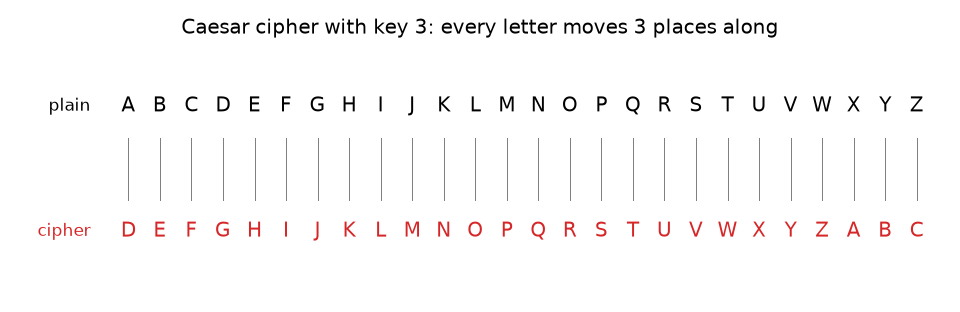
\includegraphics[width=0.85\linewidth]{figures/s01_caesar_wheel.png}\\\small Caesar cipher with key 3: each plain letter (top) becomes the letter 3 places along (bottom).\end{center}

\subsection*{E. Worked example}
Encrypt SEE YOU AT NOON with key 5, then decrypt it again.
\begin{enumerate}[nosep]
\item S = 18, 18 + 5 = 23 = X. E = 4, 4 + 5 = 9 = J. So SEE becomes XJJ.
\item Y = 24, 24 + 5 = 29, which wraps to 29 - 26 = 3 = D. O = 14, 14 + 5 = 19 = T. U = 20, 20 + 5 = 25 = Z. So YOU becomes DTZ.
\item A = 0 becomes F = 5, and T = 19 becomes Y = 24, so AT becomes FY.
\item N = 13 becomes S = 18 and O = 14 becomes T = 19, so NOON becomes STTS.
\item Ciphertext: XJJ DTZ FY STTS. To decrypt subtract 5: X = 23, 23 - 5 = 18 = S, and so on back to SEE YOU AT NOON.
\end{enumerate}
\textbf{Answer.} The ciphertext is XJJ DTZ FY STTS, and decrypting with key 5 returns SEE YOU AT NOON.

\subsection*{F. Questions}
\begin{enumerate}[nosep]
\item \textbf{Conceptual.} Why can anyone break a Caesar cipher, even without knowing the key? Does it help to keep the method secret?
\item \textbf{Numerical.} Encrypt the word GO with key 20. Show the wrap-around, then check by decrypting.
\item \textbf{Graph and simulation interpretation.} In the graph of readability against guess, why is one bar tall and the others low? Why can the gap be small for a very short message?
\item \textbf{Design and optimisation challenge.} Design: you must send a note that a classmate cannot read in the time they have, using only the ideas of this session. List two changes you could make and what each costs.
\end{enumerate}

\section{Session 2: The key space, frequency analysis and Vigenere}

\subsection*{A. Real-world problem}
Caesar has only 25 keys. A generous fix is to let the key be any rearrangement of the 26 letters: there are about 4 x 10\textasciicircum{}26 of them, far too many to try one by one. Is the cipher therefore safe? This session shows that counting keys is not enough: language has habits, and the habits leak through the cipher. You will break such a cipher by counting letters, then try to repair it with the Vigenere cipher, and finally ask how long a key must be. Everything uses toy ciphers and standard textbook results; it is not a recipe against real systems.

\subsection*{B. Concept and theory}
Key space: the number of different keys. A substitution cipher replaces each letter by another letter through a fixed rearrangement (permutation) of the alphabet, so there are 26 x 25 x ... x 1 = 26! keys. In bits, a key space of size N needs log2 N bits. Kerckhoffs's principle: a cipher should stay secure even if everything about it except the key is public, so we assume the attacker knows the method. Frequency analysis: in English, E is the most common letter (about 12.7 percent), then T, A, O, I, N. A substitution only relabels letters, so the sorted letter counts of the ciphertext are the sorted letter counts of the plaintext: matching ranks gives good guesses for the common letters. The Vigenere cipher shifts letter i by letter (i mod m) of a key word of length m, so the letter E no longer always becomes the same letter. But every m-th letter forms a column that is a Caesar cipher. The index of coincidence IC is the chance that two letters drawn without replacement from a text are equal. English gives about 0.067 (the sum of squared letter probabilities of the table is 0.0655), random letters give 1/26 = 0.038. Cutting the ciphertext into m columns gives IC near 0.07 per column only when m is the key length (or a multiple of it). For a whole Vigenere ciphertext with a random key of length m, the expected IC is 1/26 + (0.0655 - 1/26)/m. Each column must contain enough letters for its counts to show English: about 10 letters give the right shift roughly 7 times in 10, and 25 letters give it more than 95 times in 100.

\begin{itemize}[nosep]
\item N: number of keys (key space) (no unit)
\item bits: log2 N (bits)
\item m: length of the Vigenere key word (letters)
\item n: number of letters in the message (letters)
\item n\_i: how many times letter i occurs in a text (count)
\item IC: index of coincidence (no unit (0 to 1))
\item n/m: letters per column (letters)
\end{itemize}

\begin{equation*}
N_{\text{substitution}}=26!=26\cdot25\cdots1\approx4.03\times10^{26},\qquad \text{bits}=\log_2 N\approx88.4
\end{equation*}

\begin{equation*}
N_{\text{Vigenere}}=26^{m}
\end{equation*}

\begin{equation*}
\mathrm{IC}=\frac{\sum_{i}n_i(n_i-1)}{n(n-1)}
\end{equation*}

\begin{equation*}
\mathrm{IC}_{\text{whole text}}\approx\frac{1}{26}+\frac{0.0655-1/26}{m}
\end{equation*}

\begin{center}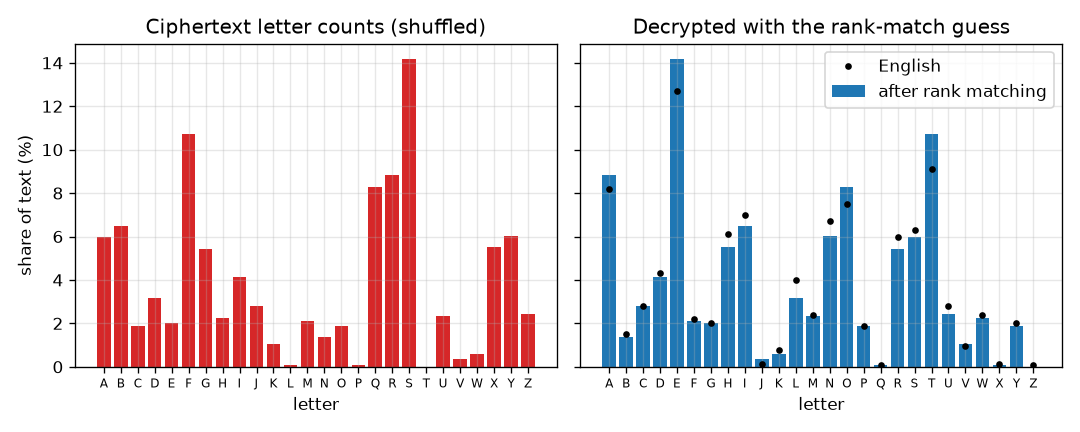
\includegraphics[width=0.85\linewidth]{figures/s02_frequency_analysis.png}\\\small Letter counts of a substitution ciphertext, and after matching ranks with English (black dots).\end{center}

\subsection*{E. Worked example}
(a) How many keys does a substitution cipher have, and how many bits is that? (b) Compute the index of coincidence of the word LETTER by hand.
\begin{enumerate}[nosep]
\item (a) 26! = 403291461126605635584000000, about 4.03 x 10\textasciicircum{}26.
\item bits = log2(26!) = about 88.4, so a brute-force search must name one of 2\textasciicircum{}88.4 keys.
\item (b) Letter counts in LETTER: L 1, E 2, T 2, R 1. Compute n\_i (n\_i - 1): L 0, E 2, T 2, R 0, sum 4.
\item n = 6, so n(n - 1) = 30 and IC = 4/30 = 2/15 = 0.1333.
\item A six-letter word is far too short to estimate IC; the answer is exact for that word but says little about English.
\end{enumerate}
\textbf{Answer.} 26! is about 4.03 x 10\textasciicircum{}26 keys (88.4 bits), and the IC of LETTER is 2/15 = 0.1333.

\subsection*{F. Questions}
\begin{enumerate}[nosep]
\item \textbf{Conceptual.} A substitution cipher has about 4 x 10\textasciicircum{}26 keys. Why is it still easy to break? What does Kerckhoffs's principle say about the attacker?
\item \textbf{Numerical.} Encrypt HELLO with the Vigenere key AB. Then say how many keys of length 3 exist.
\item \textbf{Graph and simulation interpretation.} In the figure of IC against guessed key length, why are there tall bars at 6, 12 and 18 but not at 4 or 5?
\item \textbf{Design and optimisation challenge.} Design: a message has 300 letters and you use a Vigenere cipher. Using the simulation facts of this session, choose a key length that stops the simple column attack, and give the trade-off. Why not just use a key as long as the message?
\end{enumerate}

\section{Session 3: Perfect secrecy, hashes, HMAC and key size}

\subsection*{A. Real-world problem}
Is there any cipher that cannot be broken, however much computing power an attacker has? Is a hash the same thing as encryption? How do websites check a password without storing it, and how does a receiver know that a message was not changed on the way? This session answers with toy versions of the real ideas and with numbers. Defensive education only: toy data, standard textbook results, and the clear rule that real systems must use vetted libraries, never home-made cryptography.

\subsection*{B. Concept and theory}
XOR (written \textasciicircum{}) combines two bits and is its own inverse: x \textasciicircum{} k \textasciicircum{} k = x. One-time pad: encrypt by XOR with a truly random key as long as the message and used only once. Then for the same ciphertext every plaintext of that length is possible (some key would give it), so the ciphertext reveals nothing: perfect secrecy. If a key is used for two messages, c1 \textasciicircum{} c2 = p1 \textasciicircum{} p2 and the key cancels, so the XOR of two texts is exposed; a known piece of one text then reveals the same piece of the other. A stream cipher stretches a short seed into a long pseudo-random keystream; if the seed has only b bits, an attacker tries at most 2\textasciicircum{}b seeds. Our toy generator is deliberately weak. A hash such as SHA-256 maps any input to 256 bits; the avalanche effect means one flipped input bit changes each output bit with chance one half, so on average 128 of 256 bits change, with a spread (standard deviation) of sqrt(256 x 0.5 x 0.5) = 8. Password storage: store a salted hash, hash = PBKDF2(password, salt, repetitions). The salt is random and different for every user, so equal passwords give different hashes and one precomputed table (hash to password) no longer works for all users; the attacker must hash the whole dictionary for each user. HMAC(key, message) is a hash that needs the secret key, so only key holders can make a valid tag; compare tags with a constant-time comparison so timing does not leak where they differ. Key size: trying all 2\textasciicircum{}b keys at r guesses per second takes 2\textasciicircum{}b / r seconds (half of that on average).

\begin{itemize}[nosep]
\item p, c, k: plaintext, ciphertext and key bytes (bytes)
\item b: key size (bits)
\item r: guesses per second (assumed) (guesses per second)
\item t: time to try all keys (seconds)
\item h: hash output (256 bits for SHA-256)
\item salt: random value stored with the hash (16 random bytes here)
\end{itemize}

\begin{equation*}
x\oplus k\oplus k=x,\qquad c_1\oplus c_2=(p_1\oplus k)\oplus(p_2\oplus k)=p_1\oplus p_2
\end{equation*}

\begin{equation*}
t=\frac{2^{b}}{r}\quad\text{(average }t/2\text{)}
\end{equation*}

\begin{equation*}
\text{flipped bits}\sim\text{Binomial}(256,\tfrac12):\quad \text{mean }128,\ \text{std }\sqrt{256\cdot\tfrac14}=8
\end{equation*}

\begin{equation*}
\text{tag}=\mathrm{HMAC}_{K}(m)
\end{equation*}

\begin{center}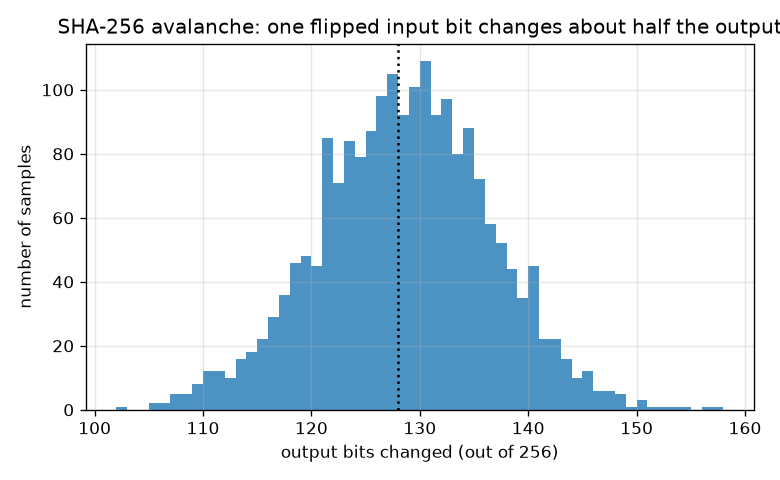
\includegraphics[width=0.85\linewidth]{figures/s03_avalanche.png}\\\small Bits changed in SHA-256 when one input bit is flipped, over 2000 random messages: centred at 128 of 256.\end{center}

\subsection*{E. Worked example}
How long does it take to try all keys of 40 bits (a) at 10\textasciicircum{}6 guesses per second and (b) at 10\textasciicircum{}12 guesses per second? How many bits are needed so that trying all keys takes at least 100 years at 10\textasciicircum{}12 per second?
\begin{enumerate}[nosep]
\item 2\textasciicircum{}40 = 1099511627776 keys.
\item (a) 1099511627776 / 10\textasciicircum{}6 = 1099512 seconds. Divide by 86400 seconds per day: about 12.7 days.
\item (b) 1099511627776 / 10\textasciicircum{}12 = about 1.1 seconds.
\item 100 years = 100 x 365.25 x 86400 = 3.156 x 10\textasciicircum{}9 seconds. Keys needed at 10\textasciicircum{}12 per second: 3.156 x 10\textasciicircum{}21.
\item log2(3.156 x 10\textasciicircum{}21) = 71.4, so round up to 72 bits. Check: 71 bits is just under 100 years, 72 bits is just over.
\end{enumerate}
\textbf{Answer.} 2\textasciicircum{}40 keys take about 12.7 days at 10\textasciicircum{}6 per second and about 1.1 seconds at 10\textasciicircum{}12 per second; 72 bits are needed for at least 100 years at 10\textasciicircum{}12 per second.

\subsection*{F. Questions}
\begin{enumerate}[nosep]
\item \textbf{Conceptual.} Why does reusing a one-time pad key destroy its security, even though the pad is perfectly secret when used once?
\item \textbf{Numerical.} A 40-bit key is tried at 10\textasciicircum{}6 guesses per second. How long does a full search take, and how does that change if the key has 41 bits?
\item \textbf{Graph and simulation interpretation.} In the time graph, which of the key sizes 40, 56, 80 and 128 bits are within one year at 10\textasciicircum{}12 guesses per second? What does the shape of the line tell you?
\item \textbf{Design and optimisation challenge.} Design: a site stores 5 users' passwords. Compare (i) plain SHA-256 hashes with (ii) salted PBKDF2 hashes against an attacker who has a table for a dictionary of 8 words. State what the attacker must do in each case and give the work.
\end{enumerate}

\section{Real-world mini-project}
\textbf{Decrypt a Vigenere ciphertext you did not write the key for.} The lesson of Session 3 generates a Vigenere ciphertext (999 letters) from a hidden key. You may use only the ciphertext and the public facts about English. First find the key length with the index of coincidence, then find each key letter with letter frequencies, and finally read the message. This is a toy exercise on data made for it; it teaches why short repeating keys are weak.

\section{The path ahead}
\begin{enumerate}[nosep]
\item \textbf{Session 4: Break a substitution cipher completely.} A solver that starts from frequency ranks and improves the key with a score for letter pairs.
\item \textbf{Session 5: Vigenere with any key length.} A Vigenere breaker that searches key lengths up to 20.
\item \textbf{Session 6: Why modes of operation matter.} A toy 8-byte block cipher used in two modes, with a pattern counter.
\item \textbf{Session 7: How strong is a password?.} A calculator for bits of entropy and the time to try every password at an assumed rate and hash cost.
\item \textbf{Session 8: Public keys with a toy RSA.} A toy RSA with the textbook numbers n = 3233, e = 17 and d = 2753, plus a trial-division factoring demo for small n.
\end{enumerate}

\section{Answers and hints}

\subsection*{Session 1}
\begin{enumerate}[nosep]
\item \textbf{Conceptual.} Hint: Count the keys, and ask what the attacker does with each one. Solution: There are only 25 useful keys, so an attacker simply decrypts with every one and reads the one that makes sense; this takes a minute by hand and a tiny fraction of a second on a computer. Keeping the method secret does not help much: the method is easy to guess, and a good cipher should stay safe even if the method is public (Session 2). All the strength must be in a key that is too numerous to try.
\item \textbf{Numerical.} Hint: G = 6 and O = 14. Add 20 and subtract 26 when you pass 25. Solution: G: 6 + 20 = 26, which wraps to 0 = A. O: 14 + 20 = 34, and 34 - 26 = 8 = I. So GO becomes AI. Check: A = 0, 0 - 20 = -20, and -20 + 26 = 6 = G; I = 8, 8 - 20 = -12, and -12 + 26 = 14 = O. Units: letter positions, no physical unit.
\item \textbf{Graph and simulation interpretation.} Hint: Think about what a wrong shift does to the letter shares. Solution: A wrong shift scrambles the message so its letters look like a random mix, scoring around the random level of about 35 percent on average; the right shift restores the real English shares, so its bar is higher (about 79 percent here against at most about 67 percent for any wrong guess). A short message has few letters, so the shares fluctuate by chance and a wrong guess can occasionally score well; longer messages give a cleaner gap.
\item \textbf{Design and optimisation challenge.} Hint: Count the possible keys, and think about what you and your friend must share beforehand. Solution: Change 1: use a different shift for different letters (for example a short repeated list of shifts). This raises the number of keys but you and your friend must now share the whole list, and Session 2 shows that short repeating lists can still be broken. Change 2: scramble the alphabet in any order, which gives far more keys, but the shape of the letter counts survives and Session 2 shows how counting breaks it. Trade-off: more keys cost more to share and remember; only a truly random key as long as the message (Session 3) gives perfect secrecy. In real life, use a vetted library, never a home-made cipher.
\end{enumerate}

\subsection*{Session 2}
\begin{enumerate}[nosep]
\item \textbf{Conceptual.} Hint: Does the attacker need to try the keys one by one? Solution: The attacker does not search the key space; the cipher leaks the letter counts, because the same plaintext letter always gives the same ciphertext letter. Matching the sorted counts with English gives the common letters at once and the rest follows from words. Having many keys is necessary but not sufficient. Kerckhoffs's principle: assume the attacker knows the method completely; only the key is secret, so the method must be strong enough to survive that.
\item \textbf{Numerical.} Hint: A = 0 and B = 1, so the shifts alternate 0, 1, 0, 1, 0. Solution: H + 0 = H, E + 1 = F, L + 0 = L, L + 1 = M, O + 0 = O, so the ciphertext is HFLMO. Keys of length 3: 26\textasciicircum{}3 = 17576 (each of 3 letters is free); the count is a pure number, and 26\textasciicircum{}6 = 308915776 for length 6.
\item \textbf{Graph and simulation interpretation.} Hint: What happens to the columns when the guessed length is a multiple of the true length? Solution: If the guessed length is 6 (or 12, 18) every column contains letters that were all shifted by the same key letter, so each column is a Caesar cipher of English and has IC near 0.07. With a wrong length such as 4 or 5, every column mixes letters shifted by different key letters, so the counts flatten and IC falls to between 0.04 and 0.055. The smallest tall bar is the key length.
\item \textbf{Design and optimisation challenge.} Hint: Compare the success rates at key lengths 8 and 20 for 300 letters, and remember what each party must remember or share. Solution: For 300 letters the column attack recovers the key in at least 90 percent of runs at key length 8 (about 37 letters per column) but in under 15 percent at key length 20 (15 letters per column). So choose a key of about 20 letters or more. Trade-offs: a long key must be shared securely and remembered or stored, and Vigenere remains a toy because other attacks and the repeating key structure still exist. A key as long as the message, random and used once, is the one-time pad (Session 3), which gives perfect secrecy but needs a fresh key for every message, which is why real systems use vetted algorithms and libraries instead.
\end{enumerate}

\subsection*{Session 3}
\begin{enumerate}[nosep]
\item \textbf{Conceptual.} Hint: XOR the two ciphertexts and see what happens to the key. Solution: c1 \textasciicircum{} c2 = (p1 \textasciicircum{} k) \textasciicircum{} (p2 \textasciicircum{} k) = p1 \textasciicircum{} p2, because k \textasciicircum{} k = 0. The key disappears and the attacker holds the XOR of two plaintexts, which still has the structure of language; if any part of p1 is known or guessed, the same part of p2 is revealed at once. The perfect-secrecy proof needs a fresh key for each message.
\item \textbf{Numerical.} Hint: t = 2\textasciicircum{}b / r. Solution: t = 2\textasciicircum{}40 / 10\textasciicircum{}6 = about 1.1 x 10\textasciicircum{}6 seconds = about 12.7 days. One extra bit doubles the number of keys, so 41 bits take about 25.5 days. Sanity check: 10\textasciicircum{}6 seconds is about 11.6 days, so 1.1 x 10\textasciicircum{}6 seconds is a little more, close to 12.7 days.
\item \textbf{Graph and simulation interpretation.} Hint: Compare each dot with the dotted one-year line. Solution: 40 bits (about 1.1 seconds) and 56 bits (about 20 hours) lie below the one-year line; 80 bits (about 38300 years) and 128 bits (about 1.08 x 10\textasciicircum{}19 years) lie far above it. The line is straight because log10 t = b log10 2 - log10 r grows by the same step for every extra bit: each bit doubles the work.
\item \textbf{Design and optimisation challenge.} Hint: How many hashes must be computed in each case, and can the table be reused? Solution: (i) Plain hashes: the attacker builds one table of 8 hashes once and finds all 5 users by lookup. In the lesson the table cracks 5 of 5 users, and equal passwords visibly have equal hashes. (ii) Salted PBKDF2: each user has a random salt, so the table finds 0 of 5 users; the attacker must compute 5 x 8 = 40 slow hashes (or more for a bigger dictionary), and equal passwords have different hashes. Trade-off: the site pays for the slow hash on every login and must store a salt per user. Salts do not protect weak passwords from a determined search; they only force the attacker to work per user. Use a vetted library and current guidance, never home-made schemes.
\end{enumerate}

\section{How to join}
Read \texttt{CONTRIBUTING.md} in the repository, then pick an issue labelled \texttt{good first issue}. Repository: \url{https://github.com/KrunalPanchal1995/opencrypto}

\end{document}
